\documentclass[10pt]{article}
\usepackage[margin=17mm]{geometry}
\usepackage{graphicx,booktabs,hyperref}
\usepackage[strings]{underscore}
\setlength{\parindent}{0pt}\setlength{\parskip}{5pt}
\begin{document}
\section*{N=58/60/100: fixed points and retained caps}
Three registered larger-variable Boolean probes, 2026-10-25.
Each uses the frozen first random-family UNSAT draw named by its input
manifest: N=58 draw 2, N=60 draw 0, N=100 draw 0. N counts Boolean variables,
not field or subgroup bits. Parameters and terminal dimensions:

\begin{center}\begin{tabular}{rrrrrrl}\toprule
N & m & field n & ell & dim at D2 & dim at D3 & D4 result\\\midrule
58 & 6 & 10 & 3 & 67 & 11,166 & allocation failed \\
60 & 5 & 15 & 3 & 74 & 18,288 & allocation failed \\
100 & 10 & 10 & 2 & 109 & 45,344 & entry cap \\
\bottomrule\end{tabular}\end{center}
\begin{center}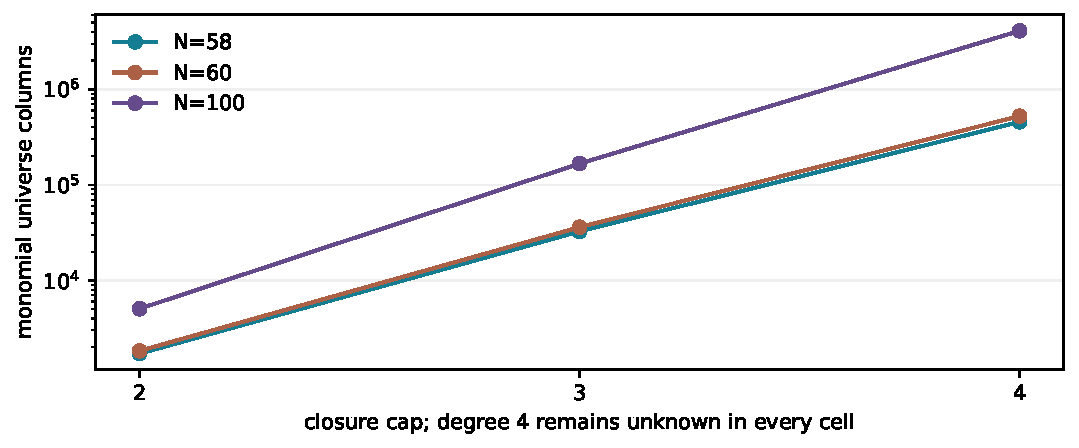
\includegraphics[width=.98\linewidth]{monomial-universes.pdf}\end{center}

All six degree-two/three closures saturate without refuting. Dense N=58 and
N=60 begin degree four and abort with allocation-failure diagnostics under
the 12-GiB address-space limit (exit 134). Sparse N=100 begins degree four
with an implicit 4,087,976-column universe, then reaches the 25-million-entry
cap (process exit 0, scientific verdict incomplete). An ordinary process exit
does not establish a fixed point. No degree-four refutation or saturation is
claimed for any cell. The sparse universe is implicit, not a dense allocation.

Limits: 900 seconds per command, 12 GiB address space, dense outer cap
600,000 columns; sparse storage has its separate entry cap. Four Rayon
threads, HKY_CHUNK=256, shared x86-64 host, L0. The u128/sparse instrument
does not remove the production library's 64-variable boundary. Dimensions
are native observations; no independent large fixed-point certificate is
provided. Exact frozen Boolean solution counts do not establish ordinary
curve/subgroup-query relevance, which remains unknown here. No bounded-degree
law, complete DLP cost, speedup or hardware result follows.

The native collector checks every input/row hash, declared variable count,
process failure and terminal status, and reproduces byte for byte.
Source: \path{examples/ic_hky_probe_summary.rs}.
Receipt: \path{../../pipeline-receipts/hky-probes-20261025/receipt.json}.
Raw archive under evidence/: \path{runs-local-followup-20261025-01.tar.xz}.
It contains all three probes and only the separate completed draw-6 pilot;
the remaining live branch campaign is not represented as finished.
Protocols: PROTOCOL.md and GUESS_CAP200K_PROTOCOL.md. The complete remote
continuation and same-input external large-cell checks remain outstanding.

\end{document}
